%---------------------------------------------------------------------------------
\chapter{Result and Discussion}
\label{chap:result}
%--------------------------------------------------------------------
We applied the contourlet HMT model for denoising and texture retrieval, and obtained promising results.

Two example are illustrated in Figure \ref{fig:petct1} and \ref{fig:petct2} as below:

\begin{figure}[h]
	\centering
	\begin{subfigure}{.5\textwidth}
		\centering
		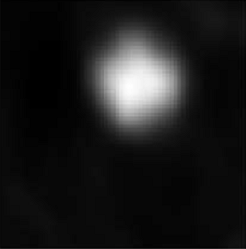
\includegraphics[width=.8\linewidth]{fig/pet1}
		\caption{PET image}
		\label{fig:sub1}
	\end{subfigure}%
	\begin{subfigure}{.5\textwidth}
		\centering
		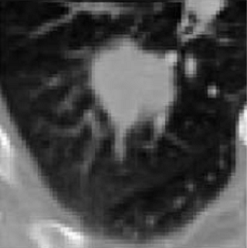
\includegraphics[width=.8\linewidth]{fig/ct1}
		\caption{CT Image}
		\label{fig:sub2}
	\end{subfigure}
	\caption{PET and CT images}
	\label{fig:petct1}
\end{figure}

\begin{figure}[h]
	\centering
	\begin{subfigure}{.5\textwidth}
		\centering
		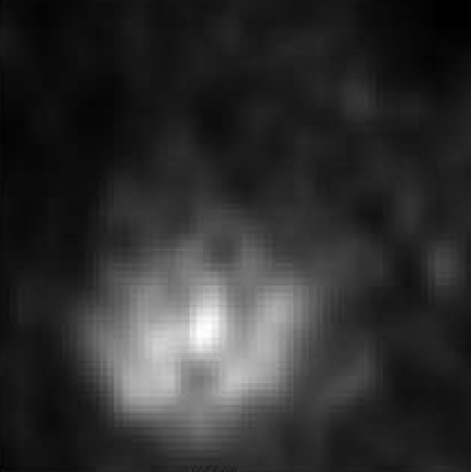
\includegraphics[width=.8\linewidth]{fig/pet2}
		\caption{PET image}
		\label{fig:sub1}
	\end{subfigure}%
	\begin{subfigure}{.5\textwidth}
		\centering
		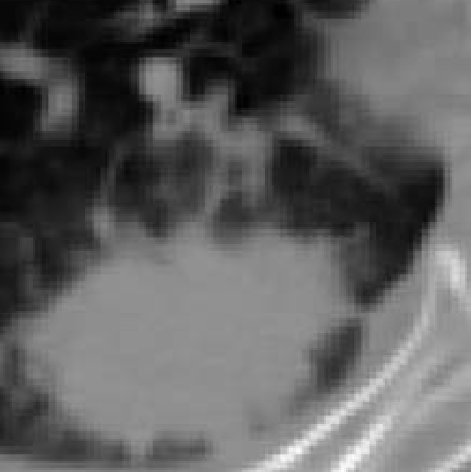
\includegraphics[width=.8\linewidth]{fig/ct2}
		\caption{CT Image}
		\label{fig:sub2}
	\end{subfigure}
	\caption{PET and CT images}
	\label{fig:petct2}
\end{figure}


In denoising, the \gls{ct} visually restores edges better than wavelet and other classical methods. It capture directional information well and offer a valuable tool in image processing. 

On the other hand, Wavelet based methods exploit observation-based transforms at different resolutions in order to better describe the whole observed information . The major drawback of Wavelets is their limited ability in capturing directional information. Consequently, an approach combining both transforms may lead to optimal performance. Our implementation combines this two methods and we achieved promising results.


The selection of the denoising technique is application dependent. So, it is necessary
to learn and compare denoising techniques to select the technique that is apt for the
application in which we are interested. By far there is no criterion of image quality evaluation that can be accepted generally
by all. A technique to calculate the signal to noise ratio in images has been proposed
which can be used with some approximation.

In this project, we have used Wavelet-Contourlet and BM3D for denoising purpose. The results can be shown in Figure \ref{fig:de1} and Figure \ref{fig:de2}. 




\begin{figure}[h]
	\centering
	\begin{subfigure}{.5\textwidth}
		\centering
		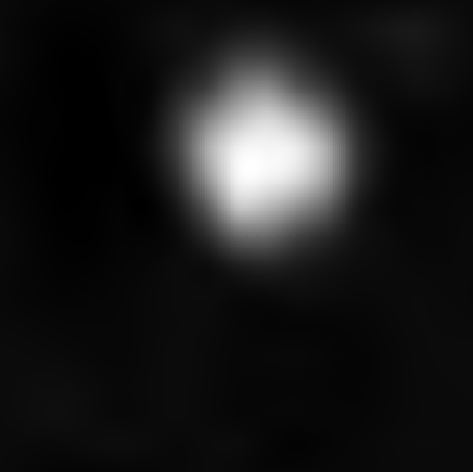
\includegraphics[width=.8\linewidth]{fig/wavelet}
		\caption{Wavelet Denoising}
		\label{fig:sub1}
	\end{subfigure}%
	\begin{subfigure}{.5\textwidth}
		\centering
		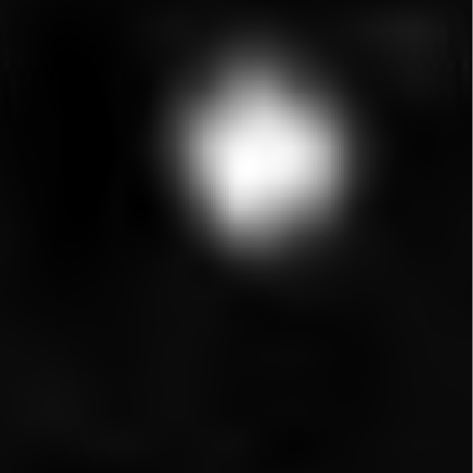
\includegraphics[width=.8\linewidth]{fig/contourlet.jpg}
		\caption{Contourlet Denoising}
		\label{fig:sub2}
	\end{subfigure}
	\caption{Wavelet and Contourlet Denoising}
	\label{fig:de1}
\end{figure}

\begin{figure}[h]
	\centering
	\begin{subfigure}{.5\textwidth}
		\centering
		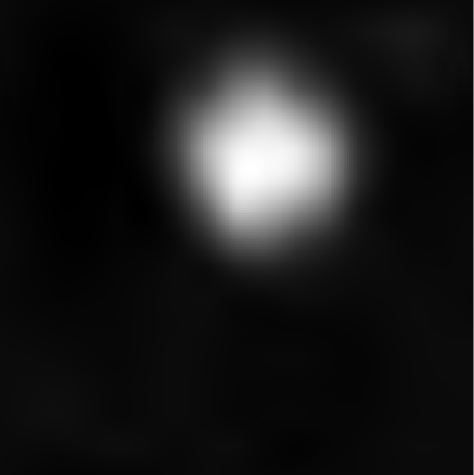
\includegraphics[width=.8\linewidth]{fig/wavecon}
		\caption{Wavelet Denoising}
		\label{fig:sub1}
	\end{subfigure}%
	\begin{subfigure}{.5\textwidth}
		\centering
		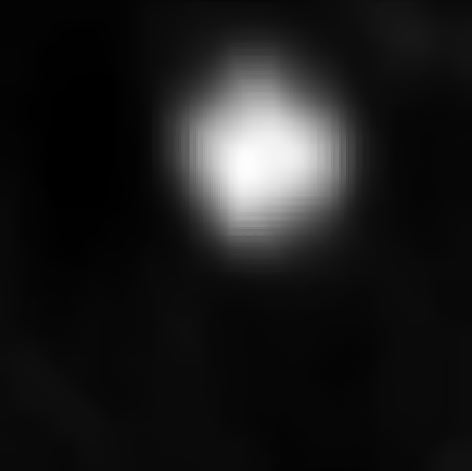
\includegraphics[width=.8\linewidth]{fig/bm3d.jpg}
		\caption{Contourlet Denoising}
		\label{fig:sub2}
	\end{subfigure}
	\caption{Wavelet-Contourlet and BM3D Denoising}
	\label{fig:de2}
\end{figure}


Image registration is the process of transforming different sets of data into one coordinate system.   It is alignment of one image
 with another. Images may be of same or different types (MR, CT, PET)

 
 In Medical imaging no single image modality provides a complete picture in all cases. Images of different modalities will infer a more comprehensive story than provided by either. So,  fusion of different modality is needed. In our implementation we have used a manual image registration using Matlab. 
 
 
 Figure \ref{fig:seg1} and \ref{fig:seg2} shows the segmented images of PET and CT.
 

 
\begin{figure}[h]
	\centering
	\begin{subfigure}{.5\textwidth}
		\centering
		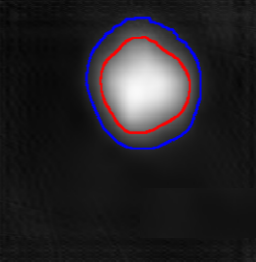
\includegraphics[width=.8\linewidth]{fig/pet1_marked}
		\caption{Segmented PET image}
		\label{fig:sub1}
	\end{subfigure}%
	\begin{subfigure}{.5\textwidth}
		\centering
		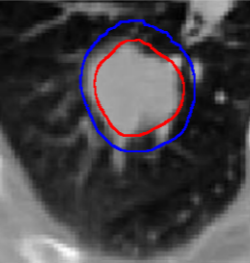
\includegraphics[width=.8\linewidth]{fig/ct1_marked}
		\caption{Segmented CT Image}
		\label{fig:sub2}
	\end{subfigure}
	\caption{PET and CT images}
	\label{fig:seg1}
\end{figure}

\begin{figure}[h]
	\centering
	\begin{subfigure}{.5\textwidth}
		\centering
		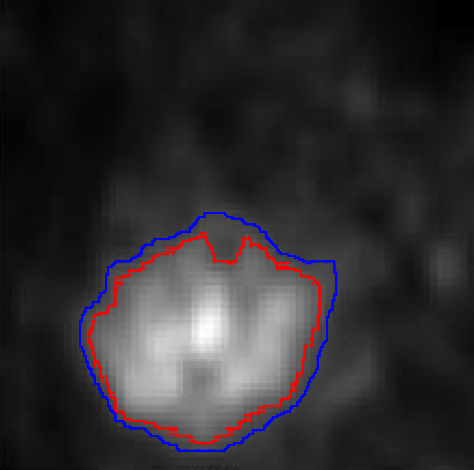
\includegraphics[width=.8\linewidth]{fig/pet2_marked}
		\caption{Segmented PET image}
		\label{fig:sub1}
	\end{subfigure}%
	\begin{subfigure}{.5\textwidth}
		\centering
		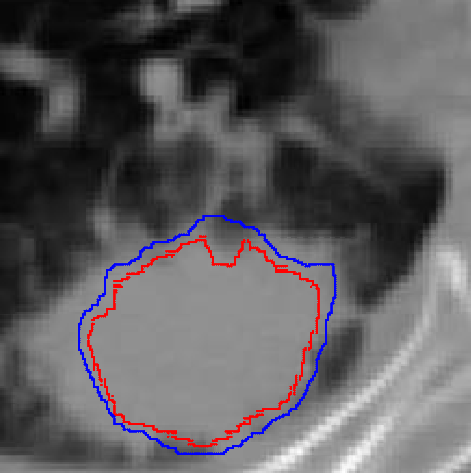
\includegraphics[width=.8\linewidth]{fig/ct2_marked}
		\caption{Segmented CT Image}
		\label{fig:sub2}
	\end{subfigure}
	\caption{PET and CT images}
	\label{fig:seg2}
\end{figure}

 In conclusion, we achieved the same results compared to the Paper.